%%%
% Automatic Layout
%%%

\section{Automatisches Layout}
\label{sec:automatic-layout}

% TODO: Verweis auf "graph-basierte Diagramme" in Begriffsklärung
Den graph-basierten Softwarediagrammen unterliegt die abstrakte Struktur des Graphen (siehe Abschnitt X). Mit der graphischen Darstellung von Graphen beschäftigt sich die mathematische Disziplin des Graphzeichnens. Ihre Aufgabe besteht darin, Layout-Algorithmen zu entwerfen, die optimale Layouts in Hinsicht auf ästhetische Regeln erzeugen, d.h. die Layout-Eigenschaften wie Position der Knoten und Routen der Kanten berechnen \cite{Eichelberger05Aesthetics, Arvo02Techniques, Siebenhaller03Automatisches}.

Unter dem automatischen Layout für graph-basierte Diagramme sind daher vollautomatische Algorithmen zu verstehen, die für ein gegebenes Diagramm die optimalen Layout-Eigenschaften berechnen und das Diagramm entsprechend anpassen.

Um während der Erstellung des Diagramms immer ein optimales Layout zu erhalten, muss der Layout-Algorithmus kontinuierlich nach jeder Änderung aufgerufen werden. Dies kann entweder automatisch oder manuell passieren.

Eine weitere Eigenschaft der Ansätze für das automatische Layout ist ein geringer Einfluss des Nutzers auf das Ergebnis des Layout-Prozesses. Oft können die Parameter des Algorithmus angepasst werden. Wenn aber die Interaktion mit dem resultierenden Diagramm unterstützt wird, hat sie keinerlei Einwirkung auf den Algorithmus und wird bei dem nächsten Aufruf des Algorithmus nicht beachtet.

Die Ansätze lassen sich in zwei Kategorien nach der Art der Sprache unterteilen, die als Eingabe für den Layout-Algorithmus verwendet wird\footnote{In der Literatur werden Ansätze für das automatische Layout meistens nach den Layout-Algorithmen kategorisiert. In dieser Arbeit richtet sich die Kategorisierung danach, wie die Ansätze zu bedienen sind und welche Art der Interaktion sie unterstützen.}. Zu einem aus einer Beschreibung eines Diagramms in einer \textbf{textuellen Sprache} unter Anwendung des Layout-Algorithmus eine graphische Repräsentation erzeugen. Weiterhin gibt es Ansätze, die auf Diagramme angewendet werden, die in einer \textbf{visuellen Sprache} modelliert sind. Diese Ansätze verändern die Layout-Eigenschaften der Diagrammelementen direkt. Beide Kategorien werden im Folgenden behandelt.

\endinput








 
\subsection{Textbasierte Ansätze}

% Eingabe != Ausgabe

Unter den textbasierten Ansätzen für das automatische Layout sind Layout-Algorithmen zu verstehen, die als Eingabe eine Beschreibung des Diagramms in Textform erfordern und als Ausgabe eine graphische Repräsentation des Diagramms liefern. Intern wird in der Regel das eingelesene textuelle Modell in ein graphisches Modell transformiert, auf das die Layout-Funktion angewendet wird. Das Resultat besitzt einen statischen Charakter und somit vermisst dieser Ansatz jegliche Möglichkeit der Interaktion. Nachträglich ändern lässt sich das Diagramm nur durch Veränderung des Quelltexts und einen wiederholten Aufruf des Layout-Algorithmus.

\subsubsection{Graphzeichnen}

% TODO: Verweis auf "graph-basierte Diagramme"
Wie bereits im Abschnitt X beschrieben wurde, bilden Graphen eine Basis für viele Typen der Softwarediagrammen. Mit der graphischen Darstellung von Graphen beschäftigt sich die mathematische Disziplin des Graphzeichnens, deren Aufgabe es ist, Layout-Algorithmen zu entwerfen, die optimale Layouts in Hinsicht auf die ästhetischen Regeln zu erzeugen \cite{Maier12A-Pattern-based}. Diese Algorithmen werden in Tools und Bibliotheken implementiert, die entweder allein stehend genutzt (siehe unten) oder in andere Programme eingebaut (siehe Abschnitt \ref{subsec:automatic-layout-graphical-approaches}) werden können.

Ein bekanntes Beispiel der Tools für die Visualisierung von Graphen ist das ursprünglich von AT\&T entwickelte Softwarepaket Graphviz\footnote{\url{http://graphviz.org}}, das in diesem Abschnitt näher beschrieben wird. Es besteht aus folgenden Komponenten:

\begin{itemize}
    \item Domänenspezifische \textbf{Sprache Dot}\footnote{\url{http://www.graphviz.org/content/dot-language}} für die Beschreibung von Graphen.
    % TODO: Bessere Beschreibung von verfügbaren Algorithmen
    \item Ein Satz von \textbf{Layout-Algorithmen}: unter anderem \textit{dot}, \textit{neato}, \textit{fdp} oder \textit{circo} \cite{Gansner14Using, NorthGansner14Dot-Manual}
    \item Ein Satz von \textbf{Kommandozeilen-Tools} für die Anwendung der Layout-Algorithmen und ihre grafische Ausgabe \cite{NorthGansner14Dot-Manual}.
    \item Eine \textbf{Software-Bibliothek}, die die Funktionalität der Layout-Algorithmen und der graphischen Ausgabe bereitstellt und sich in andere Programme einbauen lässt \cite{Gansner14Using}.
\end{itemize}

Um einen Layout-Algorithmus auf einen Graph mit Hilfe der Komandozeilen-Tools anwenden zu können, muss der Graph in der Dot Sprache beschrieben werden. Ein Beispiel eines einfachen Graphen mit 4 Knoten und 3 Kanten ist im Quelltext \ref{lst:graphviz-dot-example-dot} gegeben.

\lstinputlisting[
    caption={Beschreibung eines Graphen in Dot (\lstinline{graphviz-dot-example.dot})},
    label={lst:graphviz-dot-example-dot}
]{resources/graphviz-dot-example.dot}

Mit dem Aufruf des Befehls aus dem Quelltext \ref{lst:grapviz-dot-example-sh} wird die oben aufgelistete Dot-Quelldatei \lstinline{graphviz-dot-example.dot} eingelesen, der beschriebene Graph wird in ein internes Modell importiert, auf das der Layout-Algorithmus \lstinline{dot} angewendet wird. Anschließend wird mit dem Renderer \lstinline{png} ein Resultat in der PNG-Datei \lstinline{graphviz-dot-example.png} erzeugt, das in Abbildung \ref{fig:graphviz-dot-example} dargestellt ist \cite{Gansner14Using}.

\lstinputlisting[
    caption={Aufruf des Kommandozeilen-Tools \lstinline{dot}},
    label={lst:grapviz-dot-example-sh}
]{resources/graphviz-dot-example.sh}

\begin{figure}[hbt]
    \centering
    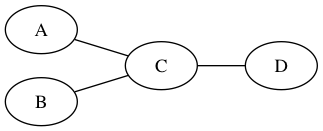
\includegraphics[scale=0.75]{resources/graphviz-dot-example.png}
    \caption{Resultat des Aufrufs des Kommandozeilen-Tools \lstinline{dot}}
    \label{fig:graphviz-dot-example}
\end{figure}

In dem diskutierten Beispiel wird sichtbar gemacht, dass das Resultat nicht interaktiv ist. Eine Änderung des Graphen ist somit nur in der Quelldatei möglich und ist mit einem wiederholten Aufruf des Komandozeilen-Tools verbunden. Aus diesem Grund ist dieser Ansatz eher für das Einbinden in automatisierte Prozesse (z.B. Generieren von Diagrammen in der automatisierten Dokumentation mit Doxygen\footnote{\url{http://www.stack.nl/~dimitri/doxygen/manual/diagrams.html}}) oder Wiki-Seiten geeignet, als für die Nutzung in einer interaktiven Umgebung.

Trotz der fehlenden Interaktivität kann das Layout von dem Nutzer beeinflusst werden, indem der Layout-Algorithmus gewählt wird bzw. seine Eigenschaften angepasst werden. Der Algorithmus kann durch die Wahl des Komandozeilen-Tools spezifiziert werden und seine Eigenschaften können zusätzlich zu der Beschreibung des Graphen in der Quelldatei angegeben werden \cite{NorthGansner14Dot-Manual}. Im oben genannten Beispiel wurde der Layout-Algorithmus \lstinline{dot} verwendet und die Richtung des Graphen in der Dot-Quelldatei mit dem Befehl \lstinline{rankdir = LR} angepasst, so dass der Graph von links nach rechts gezeichnet wird.

\subsubsection{Textbasierte UML-Tools}

Neben allgemeinen textbasierten Tools für das Graphzeichnen gibt es Tools, die für spezifische Domänen ausgelegt sind. Im Folgenden werden 2 textbasierte UML-Tools kurz vorgestellt, die aus einer textuellen Beschreibung in einer speziellen Sprache grafische UML-Diagramme erzeugen. Für die Berechnung des Layouts benutzen beide Tools intern die oben genannte Bibliothek Graphviz.

\paragraph{PlantUML}

\hyphenation{PlantUML}

PlantUML\footnote{\url{http://plantuml.sourceforge.net}} ist eine Java-Bibliothek, die für die Beschreibung von UML-Diagrammen die gleichnamige Sprache verwendet. Diese Sprache wird näher in \cite{Roques10Drawing} behandelt. Neben den vielen Anwendungen\footnote{Die bekannten Anwendungen sind unter \url{http://plantuml.sourceforge.net/running.html} aufgelistet.} bietet PlantUML einen Online-Editor\footnote{PlantUML Server: \url{http://www.plantuml.com/plantuml}} an, der es ermöglicht, UML-Diagramme direkt im Browser zu erzeugen und als Bilder zu exportieren.

\paragraph{yUML}

yUML\footnote{\url{http://yuml.me}} ist ein Online-Editor zum Erstellen von UML-Diagrammen im Browser. Im Unterschied zu PlantUML verwendet yUML eine anschauliche zeichenbasierte Sprache\footnote{Beispiele der Sprache für Klassendiagramme: \url{http://yuml.me/diagram/scruffy/class/samples}} und ist nicht in Form einer Bibliothek verfügbar. Es stellt dagegen eine HTTP-Schnittstelle bereit, so dass die Beschreibung des Diagramms direkt in eine URL-Adresse eingebettet werden kann.

\subsection{Graphische Ansätze}
\label{subsec:automatic-layout-graphical-approaches}

% Eingabe == Ausgabe

Die graphischen Ansätze für das automatische Layout unterscheiden sich von den textbasierten darin, dass der Layout-Algorithmus auf eine graphische Sprache angewendet wird. Das bedeutet, dass 

% unmittelbare Bearbeitung des Diagramms
% Ausführen des Diagramms im Nachhinein
% kein direkter Einfluss auf das Layout

%Der Layout-Algorithmus wird in der Regel erst nach der vollständigen Beschreibung des Diagramms manuell ausgeführt.

% ---

\subsubsection{Graphzeichnen in graphischen Editoren}

Wie im Abschnitt X beschrieben, bietet Graphviz eine Software-Bibliothek an, die in andere Tools eingebaut werden kann. Im Abschnitt X wurden bereits textbasierte Tools vorgestellt, die sich die Layout-Algorithmen von Graphviz zur Nutze machen. 

% Unterstützung des automatischen Layouts in OmniGraffle
% Interaktion mit dem Diagramm wird von dem Layout-Algorithmus nicht berücksichtigt => Zerstören des mentalen Modells
% Zusatzfunktion in OmniGraffle und CASE-Tools (Visual Paradigm anschauen)
% Graphviz Layout Engine

% Graphviz in Visual Paradigm

% ---

% Algorithmen für UML Klassendiagramme

% SugiBib - ein Framework, das auf dem Sugiyama Algorithmus basiert und die Semantik und Strukturregeln berücksichtigt
% https://wwwi2.informatik.uni-wuerzburg.de/SugiBib

% Kandinsky (Eiglsperger)

\subsection{Eigenschaften und Vergleich}

% Zusammenfassung
%% Verletzung der Semantik- und Strukturregeln durch die mathematischen Algorithmen
%% Interaktion im Vordergrund ist gewünscht
%% nicht geeignet für den Prozess des Zeichnens
%% Unterstützung der Diagrammtypen und deren Strukturregeln

%% Zerstören des mentalen Modells [Eiglsperger03 zitieren]
%% bei allgemeinen Algorithmen werden die Semantik- und Strukturregeln nicht berücksichtigt

%% Neuordnung des Layouts -> Zerstören der sekundären Notation [Seybold]

% Vorteile:
%% gute Ergebnisse für kleine und einfache Diagramme

% Nachteile:
%% fehlende Interaktion: Knopfdruck
%% Nutzer kann wenig beeinflussen
%% nicht für Änderungen geeignet -> Neustart
%% Semantik und Struktur...
%% berücksichtigen nicht die anwendugspezifische Einschränkungen [Gladisch]
%% Mangel an Möglichkeit der Kontrolle des Ergebnisses [Gladisch]
%% Nicht für interaktive Umgebung geeignet [Maier 2.4.1]

% Nachteile Textbasierte Ansätze:
% - fehlende Interaktion des Nutzers mit dem Diagramm
% - Veränderungen an einer anderen Stelle, keine unmittelbare Bearbeitung des Diagramms
% - geringer Einfluss auf das Layout

% textuelle Ansätze: Durch Tools interaktiv, aber an 2 Stellen!

%Die automatischen Layout-Algorithmen sind nicht für eine interaktive Umgebung geeignet. [Maier]

% nicht geeignet für Änderungen im Diagramm -> muss nochmal gestartet werden

% (deutet darauf hin, dass) -> nicht intuitiv

% im Unterschied zu [Eichelberger] beschäftigt sich diese Arbeit mit interaktiven Ansätzen, da automatisches Layout gegen Agile Modeling verstößt

% die Interaktion mit dem Diagramm fehlt (textbasierte und teilweise auch grafische)

% statisch, nicht dynamisch, nicht interaktiv

% herrausstellen

